\chapter{Przetwarzanie danych masowych na platformach\\równoległych} \label{chap.big-data-processing}

\section{Podstawowe definicje}
\subsection{Big data}
Definicja pojęcia Big data (dane masowe) jest dosyć rozległa i jednocześnie rozmyta. Świat informatyki kieruje się ku definicji iż big data występuje wszędzie tam gdzie wymagane jest przetworzenie wielkiej ilości danych. Jednocześnie nie jest zdefiniowana jednostka oraz jej wielkość od której możemy mówić o big data. Firma SAS opisuje termin big data jako: \newline \textit{"Big data is 
a  popular  term  used  to  describe  the  exponential  growth,  
availability  and  use  of  information,  both  structured  and  
unstructured"}. \newline Z kolei firma IBM big data definiuje jako: \textit{“Data, 
coming  from  everywhere;  sensors  used  to  gather  climate  
information,  posts  to  social  media  sites,  digital  pictures  
and  videos,  purchase  transaction  record,  and  cell  phone  
GPS signal to name a few”}.\cite{big_data_concept} Bazując na powyższym źródle możemy stwierdzić iż big data to zwyżkujący trend, który wskazuje na błyskawiczny przyrost danych pochodzących z różnych źródeł w krótkim okresie czasu. Jednocześnie wskazujący na znaczącą wartość danych po ich późniejszym przetworzeniu. Dla końcowego użytkownika, można uprościć, że big data to niedefiniowany zbiór różnych danych zawierający wartościowe informacje w nieuporządkowanej formie.
\subsection{4V}
W związku z mocno niedoprecyzowanym pojęciem big data publikacje naukowe definiują wymiary, które określają właściwości danych masowych.\cite{big_data_great_services} Kategorie te określa się pojęciem \textbf{4V}. Jest to skrót opisujący cztery wartości:
\begin{itemize}
	\item Objętość (Volume)
	\item Różnorodność (Variety)
	\item Prędkość (Velocity)
	\item Wiarygodność (Veracity)
\end{itemize}
Objętość wynika z samego rozmiaru danych. W założeniach są to rozmiary wielkie lecz nie można zdefiniować dokładnej wielkości oraz jednostki od której można stwierdzić iż dany zbiór danych już się kwalifikuje do zbioru big data. Brak jasno określonej wielkości ma sens ze względu na założenie, że zbiór big data jest nieskończony i stale rosnący. W związku z czym wielkość wymiaru ulega ciągłej zmianie.\newline
Różnorodność zakłada dane o nie jednorodnej strukturze. Użytkownik działający w środowisku big data jest nastawiony na dużą ilość danych, jednocześnie jest przygotowany na zorganizowanie ich samodzielnie w logiczną strukturę danych. Różnorodność to również wiele formatów danych: tekst, multimedia, grafika, dźwięk.\newline
Prędkość mówi o tempie generacji danych, które są tworzone przez wiele różnych podmiotów: ludzi, maszyn, wszelkiego rodzaju czujników. Jest to również pośrednie do samej techniki przetwarzania danych \textbf{streaming} \ref{streaming_subsection}.\newline
Wiarygodność to nic innego jak stopień poprawności danych. Wiele danych może być wygenerowanych błędnie, mogą być niekompletne, uszkodzone. Użytkownik systemu danych masowych musi samemu zdefiniować stopień do którego ufa danym na podstawie których dokonuje analizy.\newline
Ostatnim wymiarem, który nie podlega bezpośrednio terminowi 4V jest wartość (value). Jest to nie jako wypadkowa tego terminu - jaką wartość końcową stanowią dla użytkownika końcowego dane masowe. Czy wynik ich analizy przynosi realną wartość, czy koszty poniesione w stosunku do pozyskania oraz przetworzenia danych były niższe niż warość uzyskanych rezultatów?
\subsection{Klaster komputerowy}
Klaster komputerowy to najbardziej podstawowa jednostka obliczeniowa jeżeli chodzi o systemy rozproszone. Jest to zestaw połączonych między sobą samodzielnych komputerów, które mogą wymieniać wzajemnie informacji. Połączenie komputerowe opiera się o łącze o wysokiej przepustowości np. Ethernet, co gwarantuje obniżenie kosztów dystrybucji danych. Każda maszyna włączona do klastra posiada własny procesor obliczeniowy, pamięć RAM\footnote{Random access memory}, przestrzeń dyskową. Jednocześnie z punktu widzenia końcowego użytkownika, klaster posiada jeden punkt wejściowy dla obliczeń (API)\footnote{Application programmer interface}. Dzięki temu końcowy użytkownik nie jest zmuszony do zarządzania zasobami wewnętrznymi klastra i obsługuje tylko jedno źródło wprowadzania danych.\cite{cluster_grid_cloud} 
\newline Główną zaletą klastrów obliczeniowych jest wysoka dostępność. Z racji swojej rozproszonej architektury, która udostępnia łatwą skalowalność wszerz, możliwe jest dokładanie kolejnych komputerów by zwiększyć moc obliczeniową. Jednocześnie gdy moc obliczeniowa w danej jednostce czasu nie jest wymagana, komputery mogą zostać dynamicznie oddelegowane w stan uśpienia lub do innych zadań. Takie rozwiązanie jest bardzo elastyczne ze względu na potrzeby końcowego użytkownika. Dodatkowym aspektem jest stabilność klastrów. Gdy jakiś z elementów klastra ulega awarii, system monitoringu może łatwo wyszukać wadliwą jednostkę, usunąć ją z klastra i dołożyć nową, sprawną. Takie działanie pozwala użytkownikowi na korzystaniu z bardzo stabilnego rozwiązania, bez konieczności redukcji mocy obliczeniowej.\cite{cluster_grid_cloud_detailed_comparison}
\subsection{Obliczenia równoległe}
Obliczenia równoległe to rozdzielanie poszczególnych zadań dla niezależnych procesów, które z definicji posiadają osobną przestrzeń pamięci. Takie podejście jest wykorzystywane podczas przetwarzania danych masowych w klastrze komputerowym (każda maszyna jest oddzielnym procesem). Dzięki temu większość operacji jest wykonywana niezależnie co pozwala na zaoszczędzenie czasu w stosunku do obliczeń wielowątkowych, które zakładają zależność między sobą. Prof. Charles E. Leiserson wykładający na uczelni MIT\footnote{Massachusetts Institute of Technology} definuje obliczenia równoległe jako:
\newline \textit{A form of computing in which computations are broken into many pieces that are executed simultaneously}.\cite{mit_presentation}
\subsection{Obliczenia wielowątkowe}
Obliczenia wielowątkowe to rozdzielenie poszczególnych zadań między wątki aplikacji, które współdzielą przestrzeń adresową między sobą. W kontekście obliczeń w klastrze nie mają aż tak dużego znaczenia, gdyż nie gwarantują wysokiego poziomu niezależności. Wielowątkowość jest definiowana przez Prof. Charles E. Leiserson'a następująco: 
\newline \textit{A form of computing in which computations are designed as collections of interacting processes.}\cite{mit_presentation}
\section{Dostępne oprogramowanie na rynku danych masowych}
Na rynku danych masowych jest mnóstwo narzędzi, które wspierają przetwarzanie danych o dużych objętościach. Możemy podzielić je na następuje kategorie:
\begin{itemize}
	\item Eksploracja danych (Data discovery)
	\item Analityka biznesowa (Business Intelligence)
	\item Analiza bazodanowa (In-database analytics)
	\item Wysoko dostępne rozproszone zorientowane obiektowo platformy\footnote{High-availability distributed	object oriented platform - Hadoop}
	\item Zarządzanie decyzją (Decision management)    
\end{itemize}
Narzędzia z kategorii \textit{eksploracja danych} służą głównie do wydobywania informacji ze zbiorów danych o dużej objętości na podstawie danych wejściowych. Ich format jest dowolny. Często narzędzia tego rodzaju łączy się z narzędziami z dziedziny \textit{analityki biznesowej}. Dzięki takiemu podejściu można dokonywać analiz, raportów bądź pomiarów wydajności. \textit{Analiza bazodanowa} to operowanie na danych masowych po stronie bazy danych. Ta kategoria zakłada iż logika analizy danych jest zarazem częścią źródła danych. Często wykorzystywana podczas próby znalezienia relacji między danymi. \textit{Zarządzanie decyzją} - narzędzia wspomagające, bądź podejmujące decyzje na podstawie już dokonanej analizy danych. \textit{Wysoko dostępne rozproszone zorientowane obiektowo platformy} są szczególnie użyteczne podczas wstępnego przetwarzania danych. Jest to szczególnie ważne by pierwotny zbiór danych był okrojony i jednocześnie zawierał jak najwięcej wartościowych informacji. Takie podejście oszczędza czas oraz zasoby podczas bardziej złożonej analizy danych.\cite{big_data_tools}
\newline Zauważalne jest, że dane masowe mogą być przetwarzane w różnoraki sposób. Metoda analizy powinna być dobrana w zależności od potrzeb i dostępnych zasobów obliczeniowych. Ze względu na zwyżkującą popularność nowego narzędzia w kategorii \textit{Hadoop} - Apache Spark w kontekście tej pracy magisterskiej dokonane jest jego porównanie z Apache Hadoop.\cite{databricks_survey}  
\section{Paradygmat Map Reduce}
Paradygmat Map Reduce to główne założenie rozproszonego przetwarzania danych. Pomysł zrodził się w firmie Google. Internetowy gigant potrzebował łatwo skalującego się rozwiązania, które można by było zastosować do indeksowania danych, które obsługiwała wyszukiwarka. Map reduce dzięki swojej łatwej rozszerzalności i możliwości zamiany bądź usuwania poszczególnych części systemu obliczeniowego pozwolił na duże oszczędności oraz elastyczność w kwestii utrzymania systemu indeksowania. Rozszerzalność była szczególnie ważnym elementem gdyż indeksowany zbiór danych ciągle zwiększał swój zasób.
\newline
Map reduce pozwala na dzielenie dużego zbioru danych na części i wykonanie operacji na mniejszej ilości danych na danym serwerze należący do klastu komputerowego. Dzięki temu do analizy danych o dużej objętości mogą zostać zastosowane komputery o mniejszej mocy obliczeniowej, które są jednocześnie zdecydowanie tańsze w zakupie i utrzymaniu. Metoda dzieli się na dwa głowne kroki:
\begin{itemize}
	\item Map
	\item Reduce 
\end{itemize}
Krok \textbf{map} przyjmuje główną porcję danych, dzieli na mniejsze części. Następnie podzielone już porcje danych są wysyłane na poszczególne węzły(serwery) klastra komputerowego. Krok \textbf{reduce} jest odpowiedzialny za zebranie danych poddanych obróbce przez klaster. Po dokonanym kolekcjonowaniu zwracany jest wynik analizy wielkiego zbioru danych.\cite{map_reduce_description}
\newline MR\footnote{Map Reduce} możemy zapisać funkcyjnie jako:
\begin{equation}
map(k1,v1) \to list(k2,v2)
\end{equation}
\begin{equation}
reduce(k2, list (v2)) \to list (v3)
\end{equation}
gdzie \textit{map} przyjmuje problem $k1$ z dziedziny $v1$ i zwraca listę podproblemów $k2$ z dziedziny $v2$. Następnie MR zbiera wszystkie pary z tym samym kluczem $k2$ ze wszystkich list i grupuje je razem tworząc jedną grupę dla każdego klucza. Operacja \textit{reduce} jest wykonywana równolegle ($list(v2)$) dla każdej grupy. Wynikiem jest lista wartości $v3$, która może być pusta.\cite{map_reduce_microsoft_article}
\newline Przykładowa implementacja dla zliczania ilości poszczególnych słów w danym dokumencie dla języka Scala jest przedstawiona w listingu \ref{lst:scala_word_count}.
\begin{lstlisting}[language=scala, caption={Przykład "Word Count"},captionpos=b, label={lst:scala_word_count}]
//Transformacja struktury danych
val slowa = plik_wejsciowy.flatMap(linia => linia.split(" "))
// Rozdzielenie dziedziny na podproblemy
val podproblemy = words.map(slowo => (slowo, 1))
// Redukcja danych - zliczenie wystapien poszczegolnych slow
val liczba_wystapien = podproblemy.reduceByKey{case (x, y) => x + y}
\end{lstlisting}
Architektura paradygmatu MR jest przedstawiona na rysunku \ref{fig:@=map_reduce_schema}.\cite{map_reduce_figure} 
\begin{figure}
	\centering
	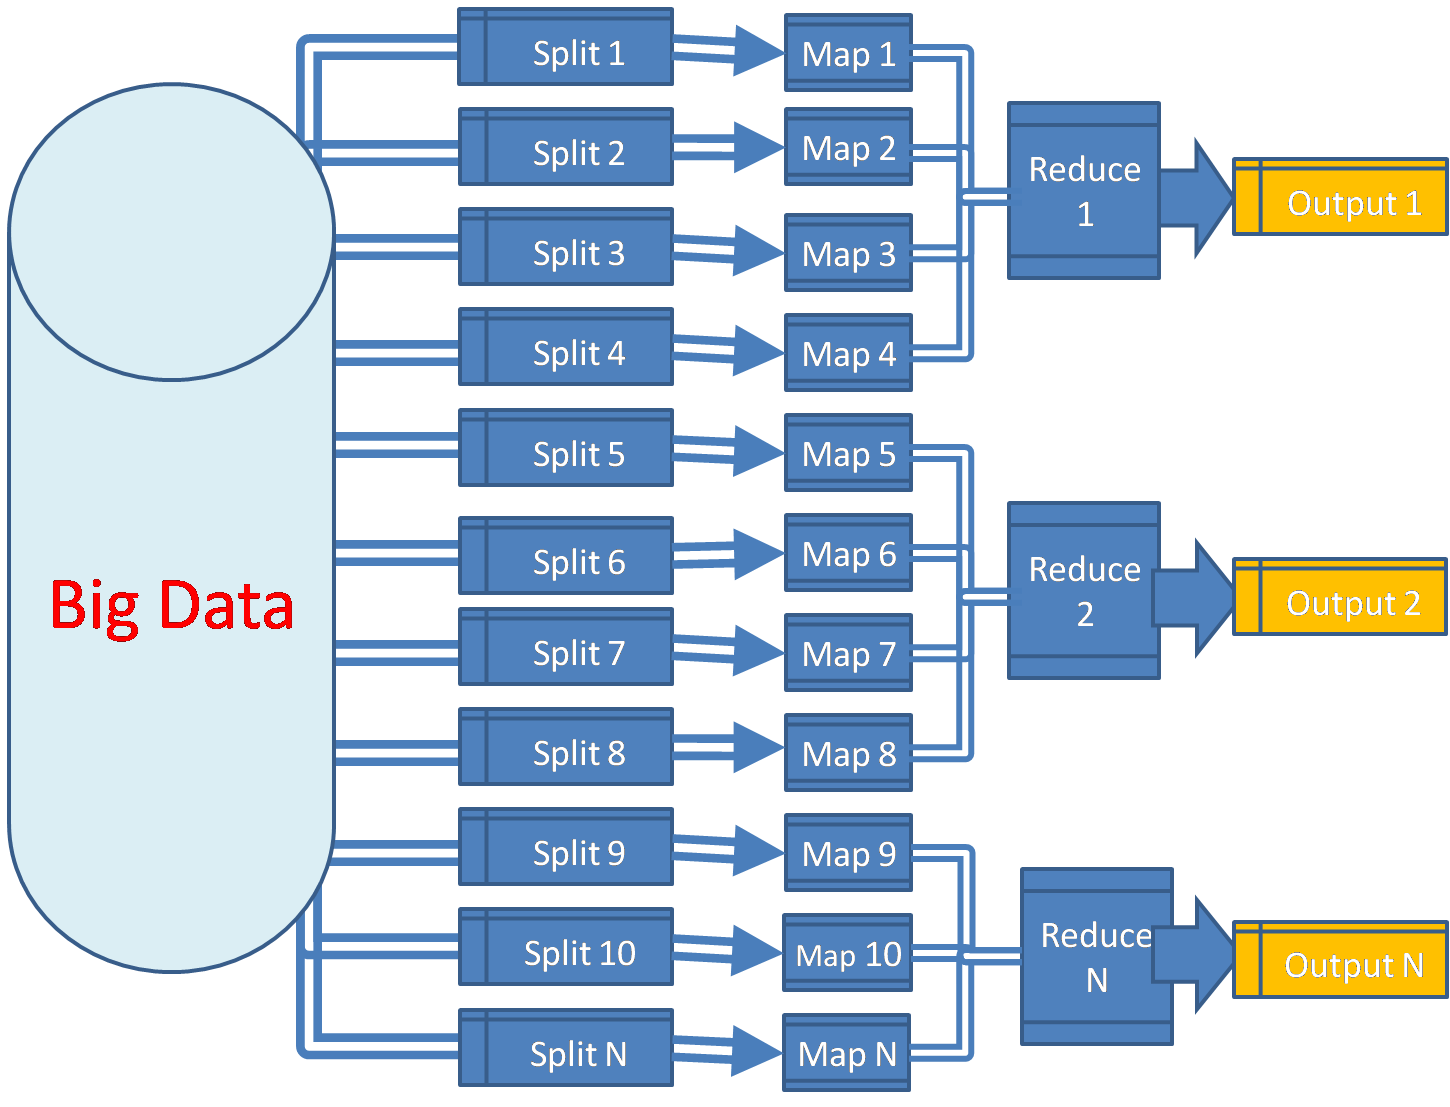
\includegraphics[scale=0.3]{map_reduce_flow.png}
	\caption{Architektura Map Reduce}
	\label{fig:@=map_reduce_schema}
\end{figure}
\subsection{Faza Shuffle w Map Reduce}
Definicja paradygmatu nic nie wspomina o fazie textit{shuffle}\footnote{tasowanie, mieszanie}. Sam paradygmat zakłada iż każdy element wychodzący z fazy map trafia do reduktora obsługującego klucz tego właśnie elementu. Oczywiście jest to przypadek idealny, który zakłada iż dane pośrednie są już posortowane bądź wszystkie elementy mają ten sam klucz (występuje jeden reduktor). W praktyce takie scenariusze nie występują często i wymagane jest zorganizowanie danych pośrednich w sposób taki by trafiły do odpowiedniego reduktora. Za tą część jest odpowiedzialna faza shuffle, która w rzeczywistości jest bardzo kosztowna gdyż sprowadza się do posortowania danych ze względu na klucz i złączenie w odpowiednie grupy na bazie klucza. Główny koszt jaki jest ponoszony to operacje wejścia-wyjścia, które są wymagane przez sortowanie i złączenie. Takie zachowanie jest widoczne na platformie Apache Hadoop.\cite{shuffle_description} Wąskie gardło paradygmatu jest ominięte w przypadku platformy Apache Spark, gdyż faza shuffle jest wykonywana w pamięci RAM co mocno redukuje koszty wejścia-wyjścia.\cite{spark_in_memory}
\newline
Praktyczna implementacja paradygmatu map reduce jest przedstawiona na rysunku \ref{fig:@=map_shuffle_reduce_schema}.\cite{map_shuffle_reduce_figure}
\begin{figure}
	\centering
	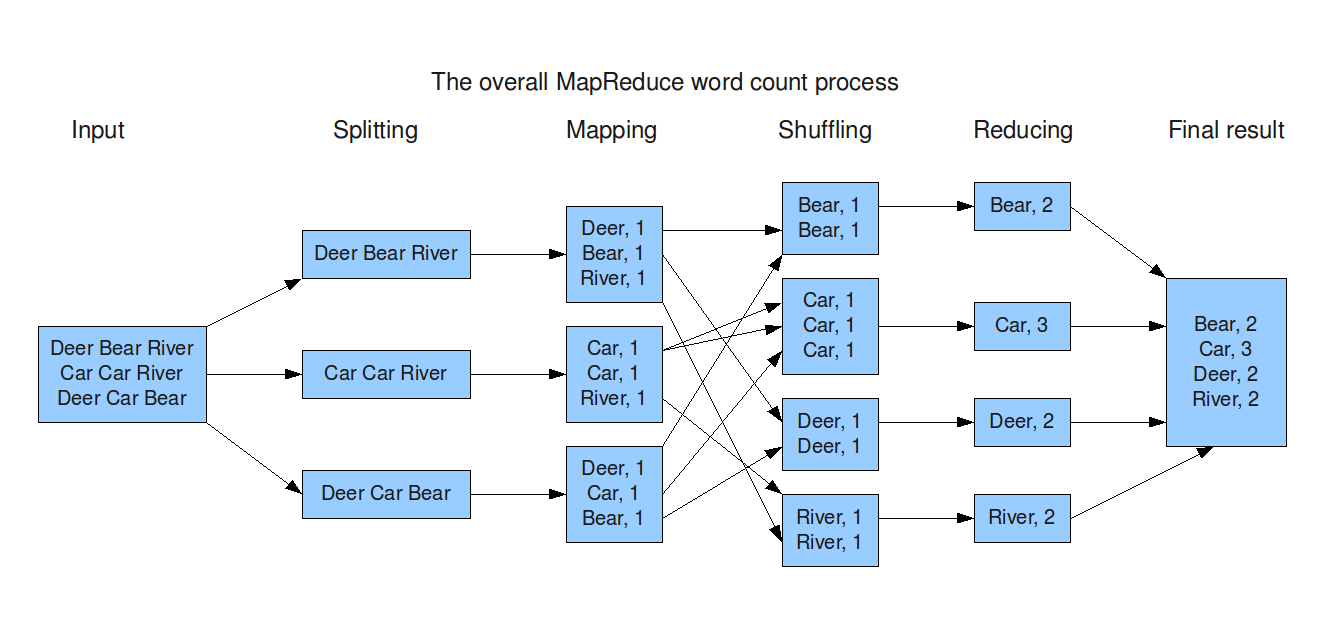
\includegraphics[scale=0.3]{MapReduceWordCount.png}
	\caption{Architektura Map Reduce wraz z fazą shuffle}
	\label{fig:@=map_shuffle_reduce_schema}
\end{figure}
\section{HDFS}
HDFS\footnote{Hadoop Distributed File System} to istotna część ekosystemów Aprache Hadoop i Apache Spark. Jest to system plików zaprojektowany specjalne do pracy w środowisku rozproszonym, którego części mogą ulegać awarii. Dzięki temu dane przechowywane w HDFS nie potrzebują kopii zapasowej, gdyż sam system z założenia dokonuje odpowiednich duplikacji. HDFS to architektura master/slave gdzie węzłem master jest jednostka o nazwie \textit{NameNode}. NameNode zawiera wszelkiego rodzaju metadane o plikach zawartych w systemie np. prawa dostępu, ilość replik. W systemie występuje jeden NameNode. Węzły slave są oznaczone nazwą \textit{DataNode} - są odpowiedzialne za przechowywanie faktycznych danych. Z racji, iż HDFS jest zaprojektowany na potrzeby danych o dużym wolumenie (od 1GB do terabajtów - dokumentacja nie definiuje konkretnej wartości) DanaNode wewnętrznie dzielą pliki na mniejsze części, które dodatkowo są duplikowane na potrzeby kopii zapasowych. HDFS jest zaimplementowany na platformie Java, także może być uruchamiany na dowolnym systemie operacyjnym. HDFS prezentuje dwa ważne założenia, które są ważne z punktu końcowego użytkownika:
\begin{itemize}
	\item Koherentność danych
	\item Przenoszenie obliczeń jest tańsze niż przenoszenie danych
\end{itemize}
Koherentność danych zapewnia łatwość w testowaniu i użytkowaniu - raz stworzony obiekt w HDFS nie zmienia swojego stanu. Jeżeli użytkownik chce zmodyfikować obiekt musi stworzyć nowy obiekt z danymi pobranymi z oryginału. Zasada przenoszenia obliczeń zapewnia zminimalizowanie transferu danych w sieci oraz poprawia ogólną przepustowość systemu.\cite{HDFS} Architektura HDFS jest przedstawiona na rysunku \ref{fig:@=hdfs_architecture}.\cite{HDFS_architecture}
\begin{figure}
	\centering
	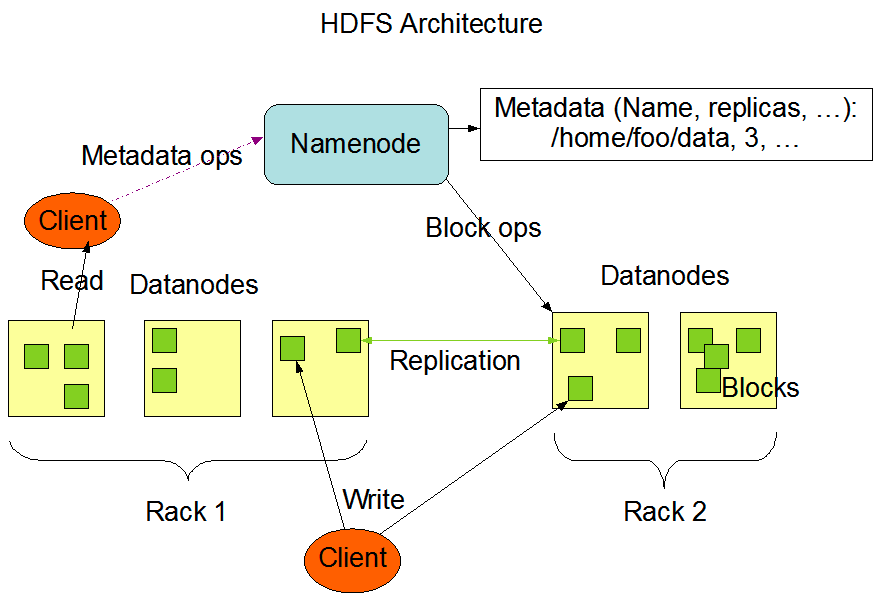
\includegraphics[scale=0.3]{hdfsarchitecture.png}
	\caption{Architektura HDFS}
	\label{fig:@=hdfs_architecture}
\end{figure}
\newline W kontekście analizy porównawczej Apache Spark i Apache Hadoop musi być zastosowany HDFS. Jest to jedyne źródło danych, na którym mogą operować obydwie platformy (Spark może pobierać dane również z innych źródeł baz typu NoSQL\footnote{Not only SQL - nierelacyjne bazy danych}).
\todo{section RDD?}
\section{Operacje - przypadki użycia w architekturze równoległej}
Występuje bardzo dużo zastosowań w przypadku analizy danych na platformach równoległych. Najpopularniejsze to:
\begin{itemize}
	\item Monitorowanie transakcji bankowych - selekcja tych transferów, które mogą być nielegalne dla pracownika banku
	\item Analiza plików logowania
	\item Analiza trendów rynkowych np. najpopularniejsze filmy w serwisie Netflix\footnote{www.netflix.com}
	\item Migracja danych między centrami w różnych lokalizacjach. Map zapewni transfer małych porcji danych w sieci, reduce zadba o złączenie wcześniej wysłanych danych oraz sprawdzenie czy nie uległy modyfikacji/regresji (np. poprzez sprawdzanie sumy kontrolnej). 
\end{itemize}